\section{Laboratory work implementation}

\subsection{Tasks and Points}

\begin{itemize}
	\item Crearea si configurarea unui ssh key
	\item initializeaza un nou repositoriu
\item configureaza-ti VCS
\item crearea branch-urilor (creeaza cel putin 2 branches)
\item commit pe ambele branch-uri (cel putin 1 commit per branch)
\item seteaza un branch to track a remote origin pe care vei putea sa faci push (ex. Github, Bitbucket or custom server)
\item reseteaza un branch la commit-ul anterior
\item folosirea fisierului .gitignore
\item merge 2 branches
\item rezolvarea conflictelor a 2 branches
\item Folosirea tag-urilor pentru marcarea schimbarilor simnificative precum release-ul.
\end{itemize}

\subsection{Analiza lucrarii de laborator}

Repository \url{https://github.com/dragosh1011/MIDPS-laboratories/tree/branch_2/MIDPS/Documentations/LAB_1}{link}

Primul pas la realizara acestei lucrai de laborator a fost configurarea unei ssh key. Pentru aceasta am folosit documentatia de pe github \cite{ssh-key} care ofera pas cu pas informatia cum se realizaza acest lucru. 
Realizarea unui repositoiu am facut-o pe interfata web a githab. Github ofera comanda \hl{git config} pentru a configura numele si emailul utilizatorului.


Pentru crearea un branch si schimbrarea imediata pe acesta am utilizat \hl{git checkout -b}, iar apoi pentru schimbarea pe un branch existent \hl{git checkout}. Pentru a face commit si push pe remote branch am utilizat \hl{git commit -am message} si \hl{git push origin branch}. 

\hl{git reset HEAD\~} ofera posibilitatea de a te anula utlimul commit realizat. File-ul .gitignore se gaseste aproape in orice repozitoriu git, deoarece majoritatea proiectelor in procesul de dezvoltare utilizeaza multe fisiere care nu sunt relevante pentru fiecare dezvoltator sau contine fisiere ce sunt specifice pentru fiecare dezvoltator in parte. \hl{git merge branch} este comanda care permite sa facem merge intre branchul actual si un branch remote. 

Rezolvarea conflictelor este o necesitate des intilnita atunci cand la un proiect lucreaza mai multi dezvoltatori concomitent. Chiar si daca esti un singur dezvoltator, nu esti scutit de riscul de a avea la un moment dat conflicte, daca nu ai tinut cont de unele modificari facute pe alte branchuri. Tagurile sunt intilnite apropae in oricare proiect, deoarece este important de creat o versionare a produsului care permite urmarirea modificarilor care se fac de la o veriune la alta, dar si revenirea la o versiune mai veche in caz de necesitate.

\subsection{Imagini}

\begin{center}
	\begin{figure}[h]
		\centering
		
\includegraphics[width=10cm]{ssh}\\
		\caption{Configured ssh key}
		\label{run}
	\end{figure}
	
	\begin{figure}[h]
		\centering
		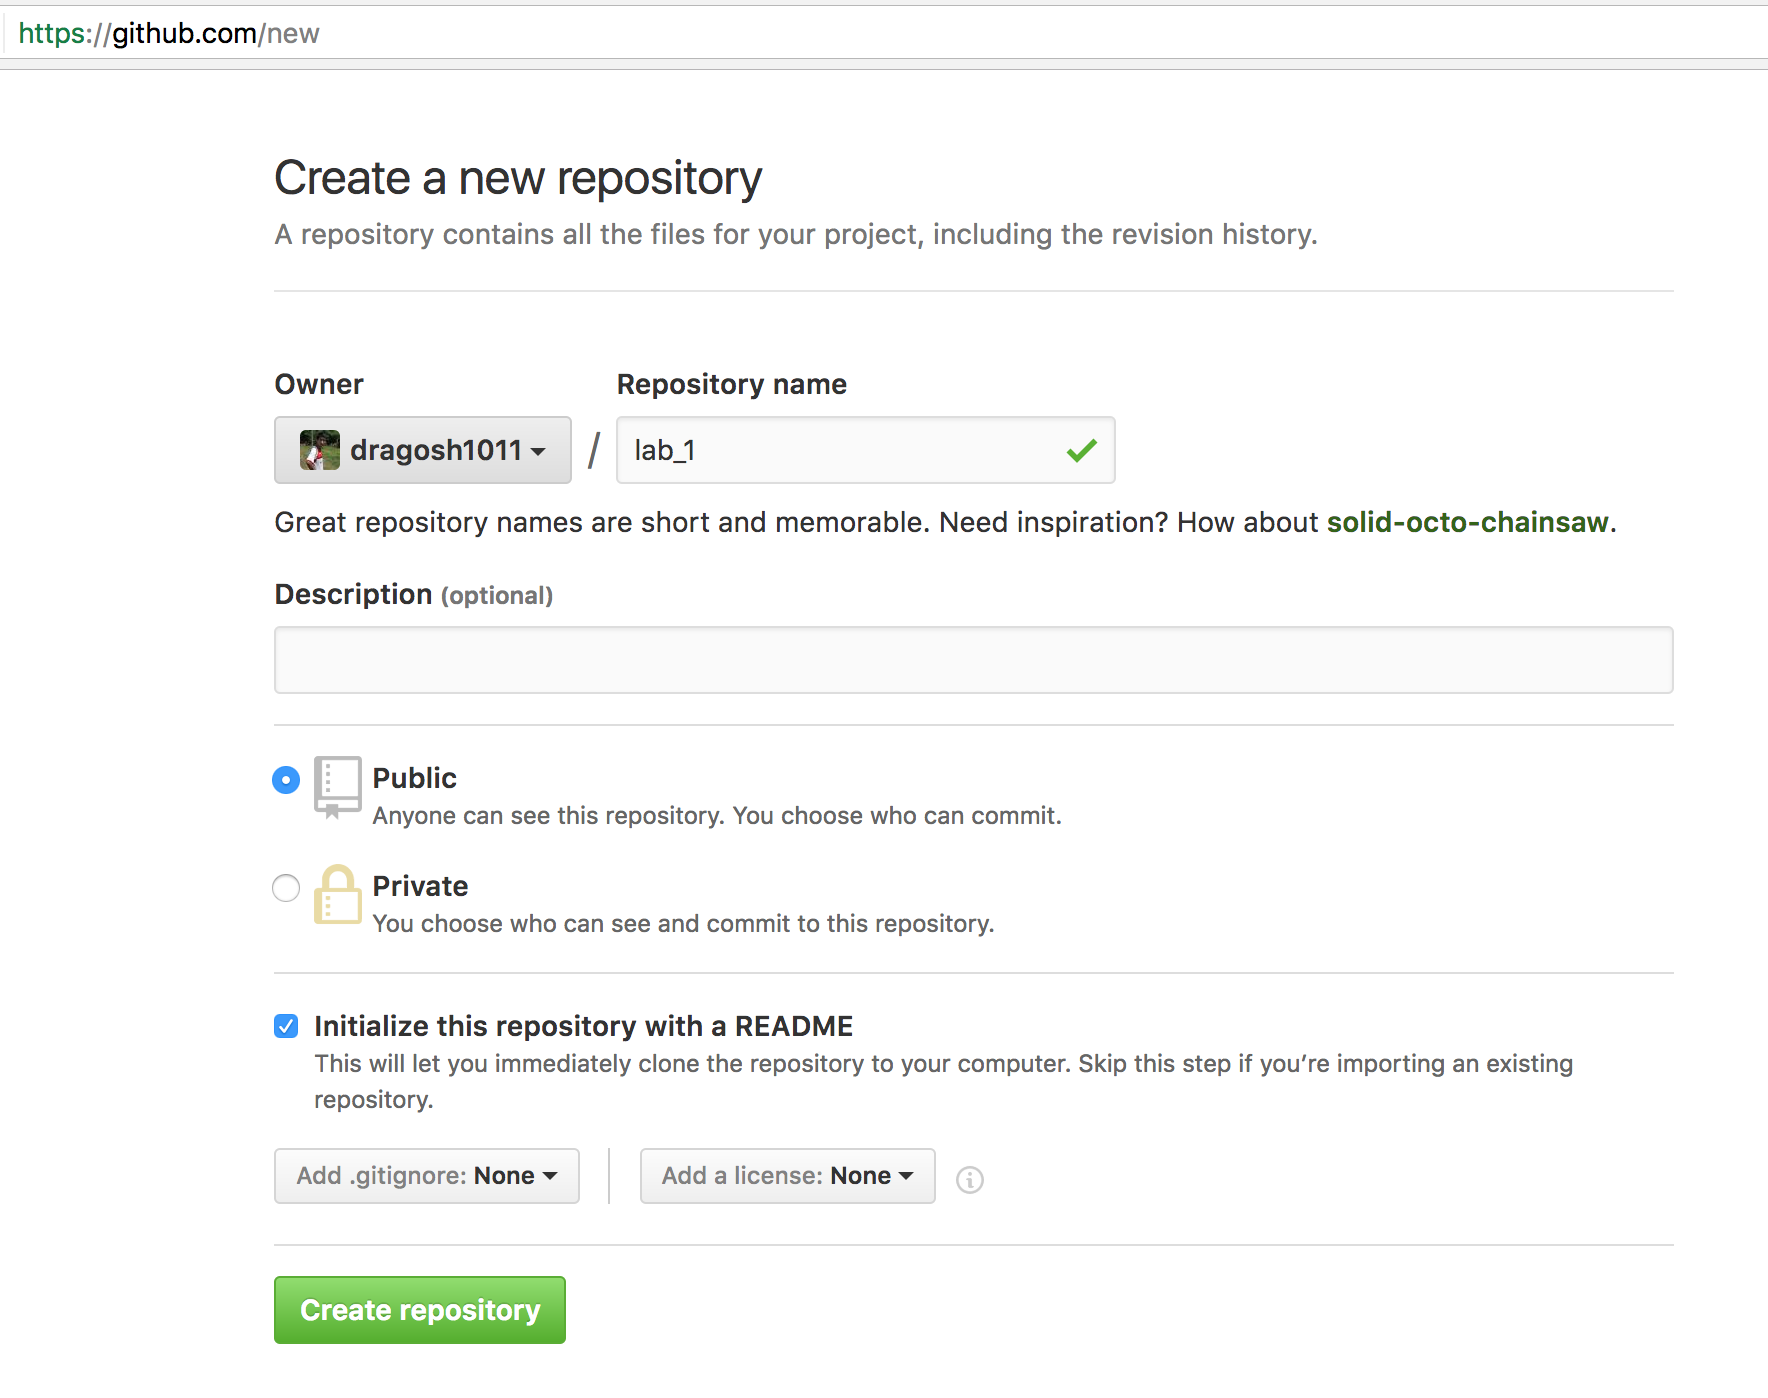
\includegraphics[width=10cm]{new-repo}\\
		\caption{Create new repository}
		\label{jump}
	\end{figure}
	
	\begin{figure}[h]
		\centering
		
\includegraphics[width=10cm]{config}\\
		\caption{Config github user name and email}
		\label{slide}
	\end{figure}
	
	\begin{figure}[h]
		\centering
		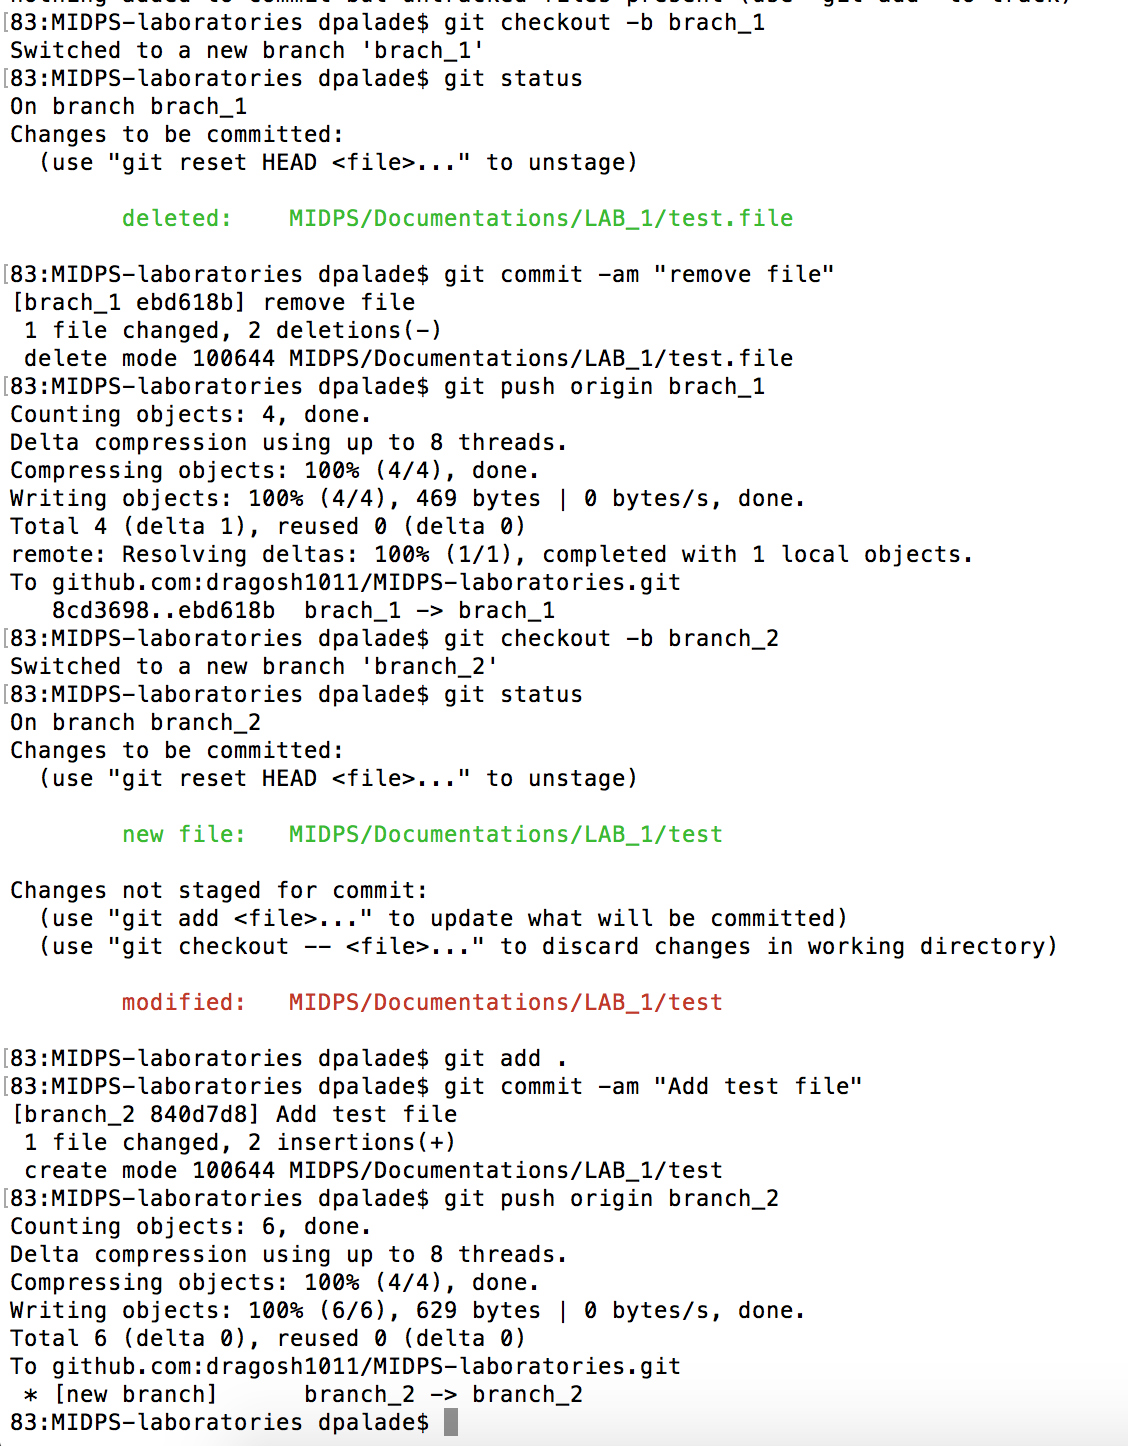
\includegraphics[width=10cm]{branches}\\
		\caption{Create 2 branches and do commits on them}
		\label{run}
	\end{figure}
	
	\begin{figure}[h]
		\centering
		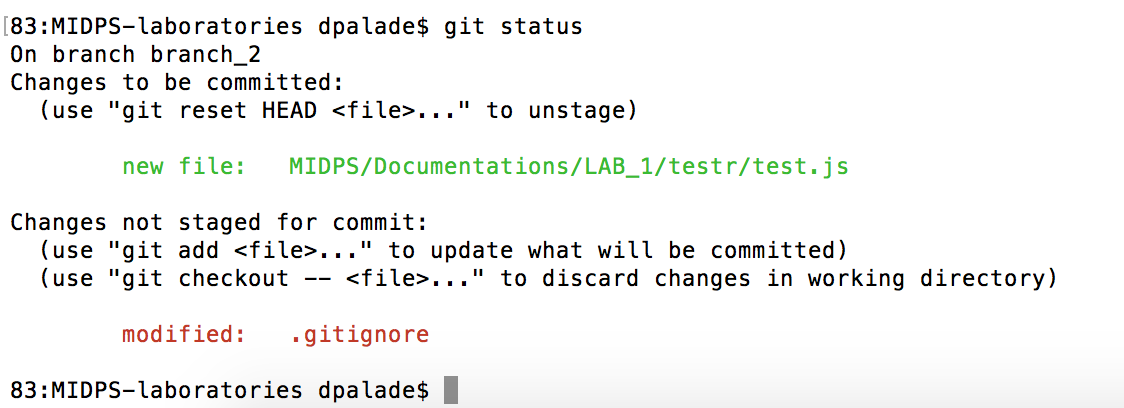
\includegraphics[width=10cm]{gitignore}\\
		\caption{Use .gitignore}
		\label{jump}
	\end{figure}
	
	\begin{figure}[h]
		\centering
		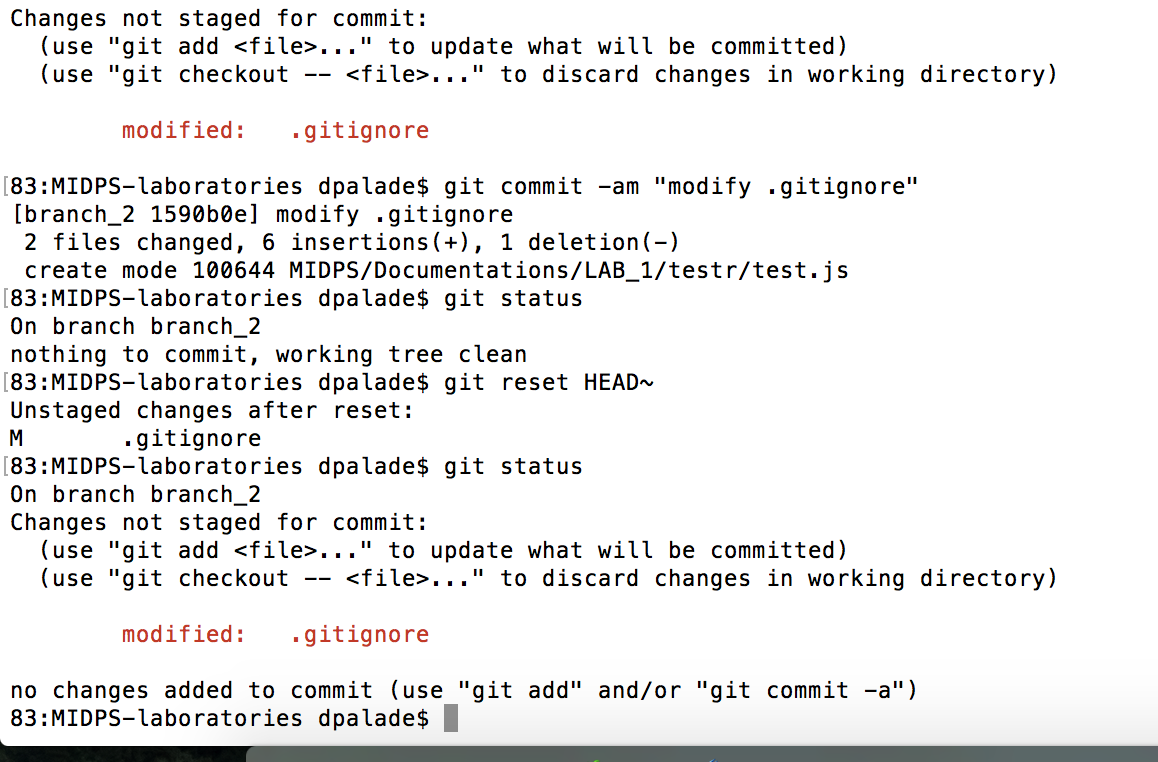
\includegraphics[width=10cm]{reset-commit}\\
		\caption{reset last commit}
		\label{slide}
	\end{figure}
	
	\begin{figure}[h]
		\centering
		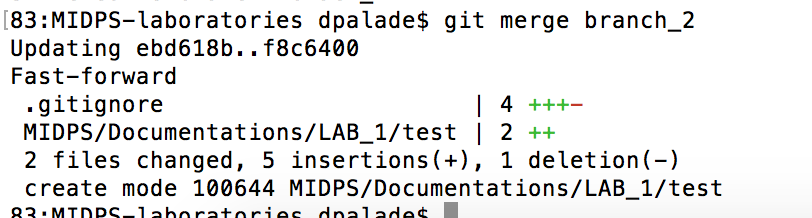
\includegraphics[width=10cm]{merge}\\
		\caption{Merge 2 branches}
		\label{run}
	\end{figure}
	
	\begin{figure}[h]
		\centering
		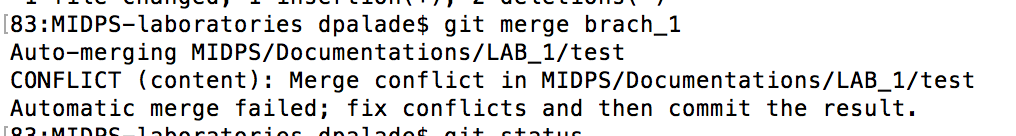
\includegraphics[width=10cm]{conflict}\\
		\caption{Conflict}
		\label{jump}
	\end{figure}
	
	\begin{figure}[h]
		\centering
		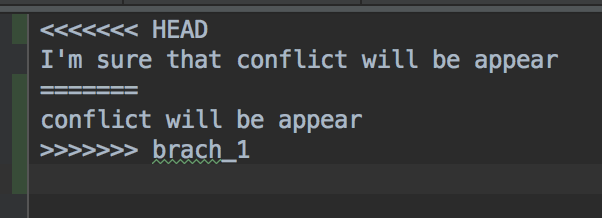
\includegraphics[width=10cm]{conflict-file}\\
		\caption{Conflict file}
		\label{slide}
	\end{figure}
	
	\begin{figure}[h]
		\centering
		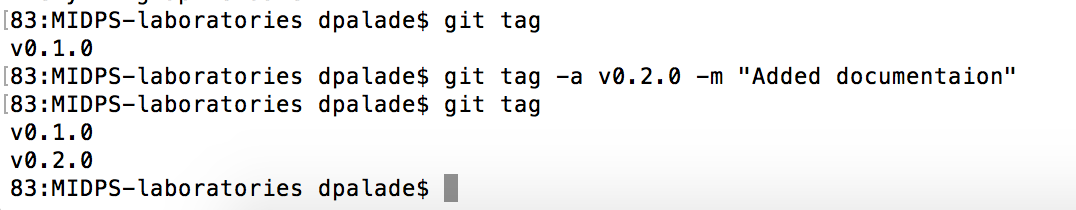
\includegraphics[width=10cm]{tag}\\
		\caption{Tag}
		\label{slide}
	\end{figure}
\end{center}

\clearpage